\documentclass{article}
\usepackage[utf8]{inputenc}
\usepackage{array,multirow,graphicx}
\usepackage{amsmath,amssymb,latexsym}
\usepackage{mathabx}
\usepackage{parskip}
\usepackage{listings}
\usepackage[section]{placeins}
\usepackage{hyperref}
\usepackage[english]{babel}
\usepackage{biblatex}
\renewcommand{\sfdefault}{ptm}
\graphicspath{ {/} }

\title{Report.6.Subquery}
\author{Linh Duong}
\date{November 2017}

\begin{document}

\maketitle

\section{What is the average salary of each employee?}
\begin{lstlisting}[language=sql]
select distinct employees.emp_no,concat(first_name,' ',last_name) 
as fullname
from employees join dept_emp on employees.emp_no=dept_emp.emp_no 
join departments on departments.dept_no=dept_emp.dept_no
where last_name in (select last_name 
from employees 
join dept_manager on employees.emp_no = dept_manager.emp_no
join departments on departments.dept_no=dept_manager.dept_no 
and dept_name='Finance');
\end{lstlisting}
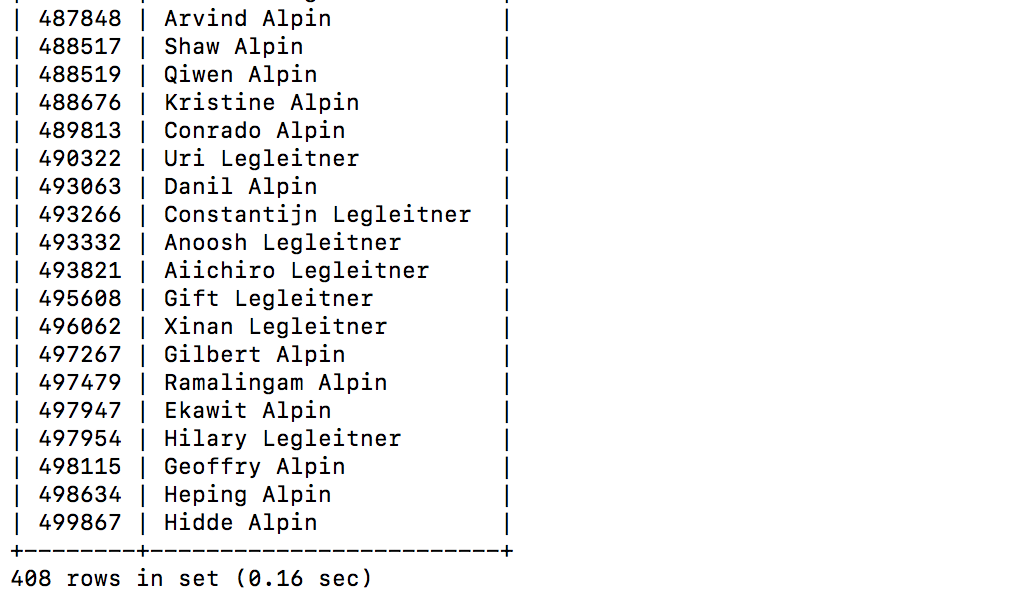
\includegraphics[width=\linewidth]{1.png}

\section{How much was each employee paid in total?}
\begin{lstlisting}[language=sql]
select employees.emp_no, concat(first_name,' ',last_name)
as fullname
from employees join dept_emp on employees.emp_no=dept_emp.emp_no 
join departments on departments.dept_no=dept_emp.dept_no 
and dept_name='Production'
where from_date > ( select from_date from dept_manager 
where dept_no = (select dept_no from departments 
where dept_name='Production') 
order by from_date desc limit 0,1);
\end{lstlisting}
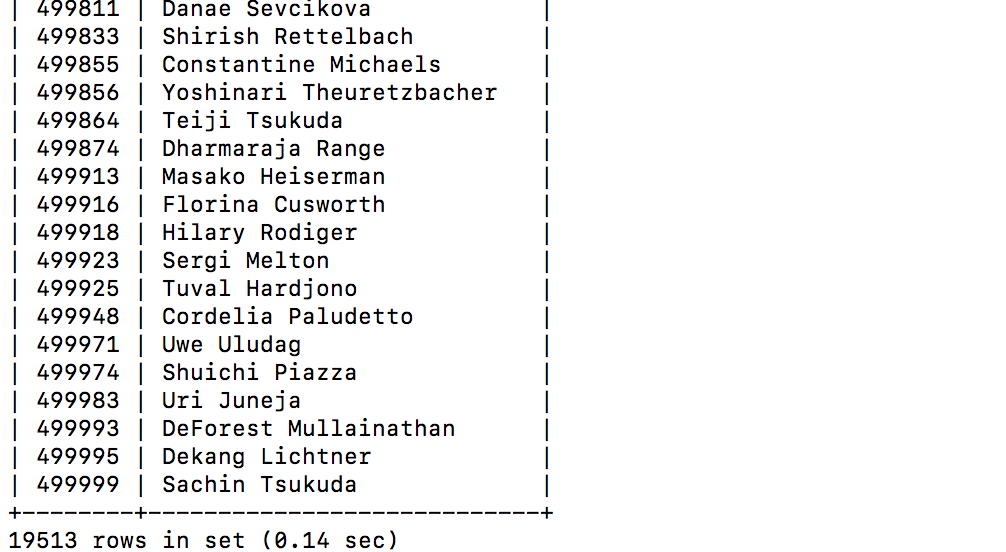
\includegraphics[width=\linewidth]{2.png}

\section{Minimum, maximum and total salaries of each department?}
\begin{lstlisting}[language=sql]
select dept_name, average from 
(select dept_emp.dept_no, dept_name, avg(salary) as average 
from salaries join employees on employees.emp_no=salaries.emp_no 
join dept_emp on dept_emp.emp_no = employees.emp_no
join departments on dept_emp.dept_no = departments.dept_no
group by dept_emp.dept_no ) as average1
order by average desc;
\end{lstlisting}
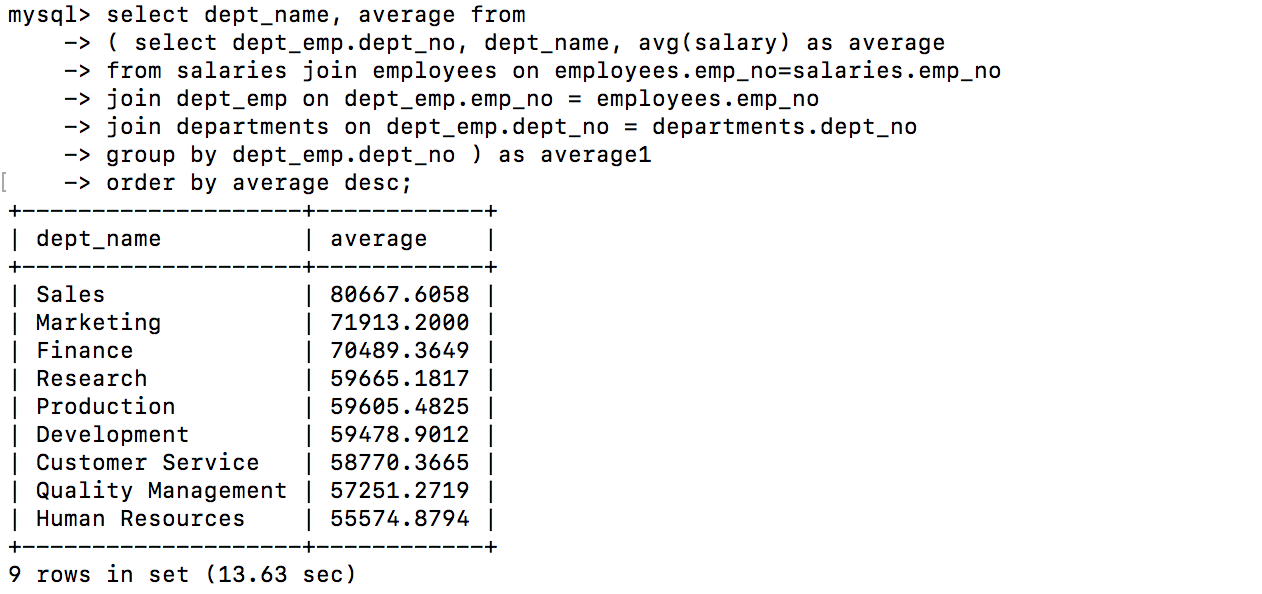
\includegraphics[width=\linewidth]{3.png}

\section{Which departments have paid more than 20 billion dollars for their employees?}
\begin{lstlisting}[language=sql]
select title, avg(salary) as average 
from salaries join employees on employees.emp_no=salaries.emp_no 
join titles on employees.emp_no = titles.emp_no
where title in (select distinct title 
from titles where title like '%Engineer%')
group by title
order by average desc;
\end{lstlisting}
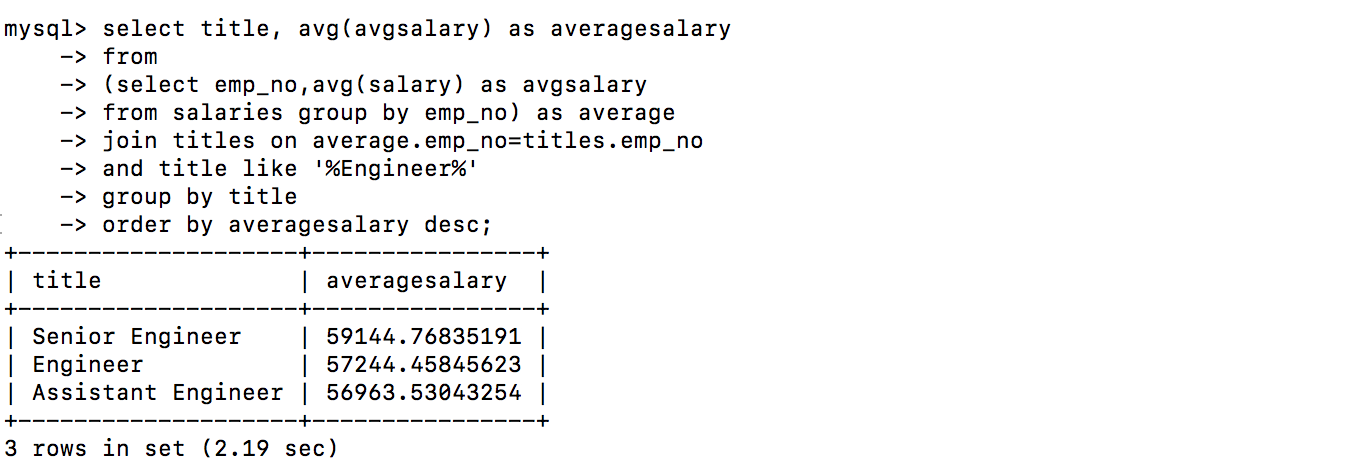
\includegraphics[width=\linewidth]{4.png}


\end{document}